\documentclass[11pt]{article}
\usepackage{fullpage}
\usepackage{float}
\usepackage{amsmath}
\usepackage{graphicx}
\graphicspath{./images/}
\title{CS63 Spring 2019\\Looking for the Right Sign: Using Convolutional Neural Networks on American Sign Language (ASL)}
\author{Mickey Haregot and Chris Zhang}
\date{05/03/2019}

\begin{document}

\maketitle

\section{Introduction}


It is expected that anyone who has learned about deep learning has been introduced to the MNIST data set example. The applications of deep learning on similar data sets have been shown to be extremely useful in aspects such as zip code recognition on letters or dollar amounts on checks. Deep learning has been applied not only to digits but also to letters. For this paper these letters will not be written letters but rather signed letters. The majority of the American population is not fluent in ASL, as around 10\% of the population have some degree of hearing loss, according to Start ASL. Also, sign language is not an international language. As little people know sign language and sign language varies from region to region, communication between deaf and speaking communities is often a complicated process. Substituting for other forms of communication, such as written communication, is inconvenient and would barely compare to the speed at which two speaking or signing people could communicate with each other. The intention of this paper is to use deep learning, particularly convolutional neural networks (CNNs), to analyze images of signed letters as a means to contribute to the improvement of communication between deaf and hearing communities. Issues to note are that, as we are using images, non-static letters such as 'j' and 'z' are excluded from both training and testing data sets. Below are the colorized and uncolorized - the latter is used in the data set - images of signs in the the Sign Language MNIST data set. \\
\begin{figure}[H]
\begin{center}
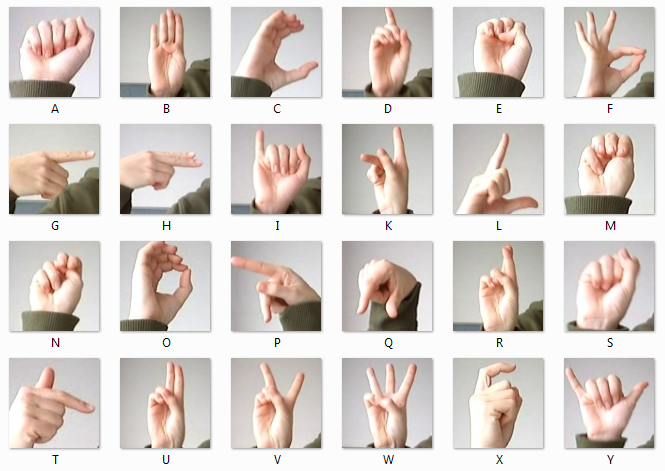
\includegraphics[scale=0.44]{images/amer_sign2.png}
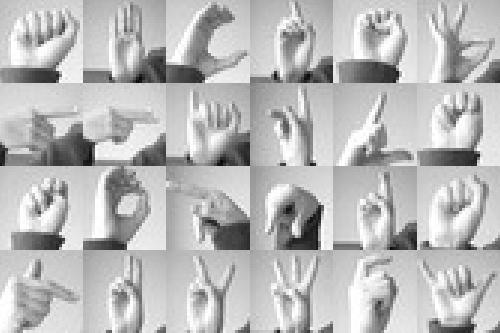
\includegraphics[scale=0.62]{images/amer_sign3.png}
\caption{Top: ASL Alphabet Sign Images, Bottom: Uncolorized and Simplified Data Set Images}
\end{center}
\end{figure}

Convolutional neural networks are a particular tool within deep learning that work most effectively on data that contains spatial relationships in two dimensions (2D). As our data are composed of pixel values for 2D images of ASL signs, we decided to use a CNN in order to build a network that identified features in these images in order to predict what letter of the alphabet the sign represents.

\section{Method and Details}

\par
The data set used for this project comes from a Kaggle competition titled "Sign Language MNIST" (the URL for this competition: https://www.kaggle.com/datamunge/sign-language-mnist/version/1). The data set provided was derived from a smaller set of 1704 colored images of hands forming the alphabet from American Sign Language, excluding the letters 'j' and 'z'. These images were then modified with the use of an image pipeline based of off ImageMagick, a free and open-source software used for displaying, converting, and editing raster image and vector files. Modifications consisted of five percent randomization of pixels, fifteen percent increases and decreases in brightness and contrast, and rotations on the images. The modifications resulted in a training data set of 27,455 and a testing data set of 7,172 images The images were represented in 28x28 form of 784 pixels, each pixel taking on a value between 0 and 255. This matches the dimension of the original MNIST data set, which is also made up of 784-pixel sized images.

The ASL data came in two .csv files: one containing training data and the other containing testing data. In each spreadsheet, each row represented an image or data point. The first column contained the label for each row/image, where the label took on a value between 0 and 24 (inclusive of endpoints and excluding 9) and represented the index of a letter in the English alphabet. The second column contained the pixel values for each image; there were 784 columns beyond the first column containing each image's label. Each of those pixel value columns contained a value between 0 and 255. In order to process these data, for both training and testing sets, we had to read in each line of a data file, appending each row's label to a label vector and appending each column's pixel value into an array of pixel values, and then appending the latter array - which represented one image's 784 pixel values - to an array of all images' pixel values.

After pre-processing the raw .csv data, we constructed a CNN, identical - in terms of layers and data size - to the network that we used in-lab for the MNIST data set during Lab 8. We adjusted this neural network to produce output that took form as an array of length 25, using one-hot representation to indicate which letter the network predicted. From there, the one-hot representation was converted to an integer value, representing the index of the letter in the English alphabet that the network predicted. This predicted index was compared against the respective target from the target vector of labels. This CNN was composed of a 2D Convolutional Layer, a 2D Pooling Layer, a Flatten layer, and two Fully-Connected/Dense Layers. Although this was the CNN setup used for MNIST, we wanted to construct an alternate CNN that may improve accuracy on the ASL MNIST data set.

This second, or "new" CNN, was based off of the network outlined during in-class lecture (Lecture 10A, Slide 12). This CNN's structure was similar to that of the "old" CNN, except it used an extra pair of a 2D Convolutional Layer and a 2D Pooling Layer. We expected this new CNN to acheive a higher accuracy rate, on average, than the old CNN due to this extra pair of Convolutional and Pooling layers, which help the network learn features more robustly.

In terms of both parameters, both our old and new CNNs were identical. The optimizer function was Stochastic Gradient Descent (SGD), which used a default learning rate of 0.01, according to Keras documentation. The loss function was categorical\_crossentropy, which was appropriate for the one-hot representation we used to categorize what letter an image featured. Our metric was accuracy, as we sought to achieve the highest accuracy rate in using our CNN to predict the letter an image and its featured sign was showing. Our activation functions were all RELU, except for the last fully-connected layer in which the activation function was softmax.

For our first CNN that was based on the example network from Lab 8, our old CNN, we used two charts to optimize the epoch count for our network's training. The first chart, titled \textit{Model Loss}, plotted Loss (for both training and testing data) against Epoch count. We created this chart for 100 epochs and noticed that Loss for testing/validation data was minimized at 10 epochs, after dramatically decreasing with each additional epoch from 0 to 9 epochs. Beyond 10 epochs, however, the Loss value increased slightly with each additional epoch. This identified 10 epochs as the optimal epoch count for our first network; epoch counts beyond 10 leads to over-fitting/training, which is detrimental to our network's ability to correctly categorize images of ASL signs for novel, testing data.

The second chart we used was titled \textit{Model Accuracy} and plotted Accuracy (for both training and testing data) against epoch count. We created this chart for 100 epochs and noticed that Accuracy for testing data reached an apex at 10 epochs, after increasing dramatically with each additional epoch from 1 to 10 epochs. From 10 to 100 epochs, the Accuracy stayed relatively flat; it didn't improve or worsen. This coupled with the insight from the \textit{Model Loss} chart, we determined that 10 epochs was optimal for this CNN, as prediction accuracy is at a maximum and value loss is at a minimum, for training/validation data, at 10 epochs. Below are pairs of \textit{Model Loss} and \textit{Model Accuracy} charts for 100, 25, and 10 epochs:

\begin{figure}[H]
\begin{center}
    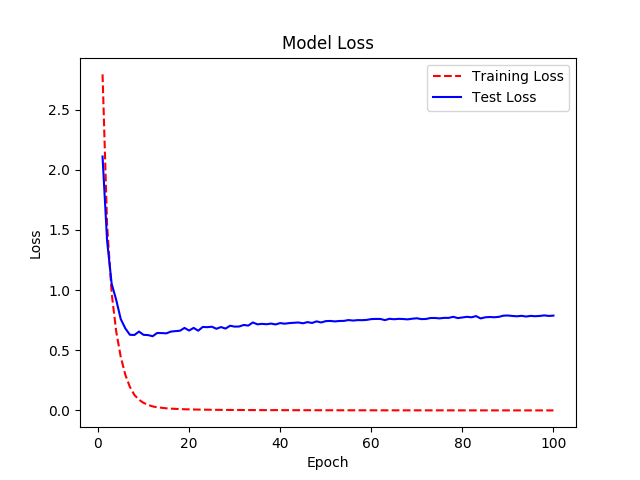
\includegraphics[scale=0.5]{images/OldModelLoss100Epochs.png}
    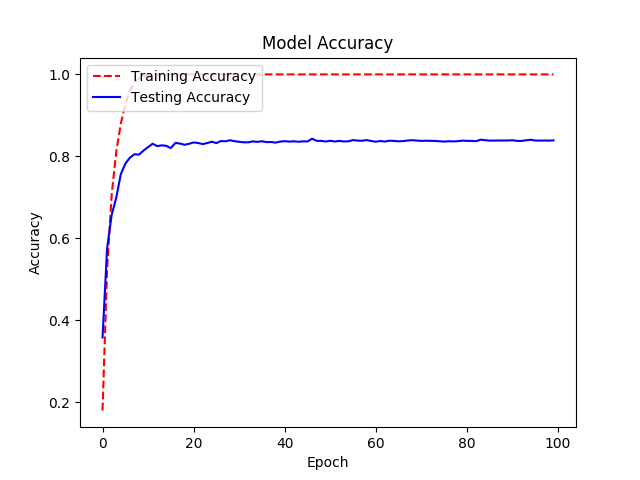
\includegraphics[scale = 0.5]{images/OldModelAccuracy100Epochs.png}
    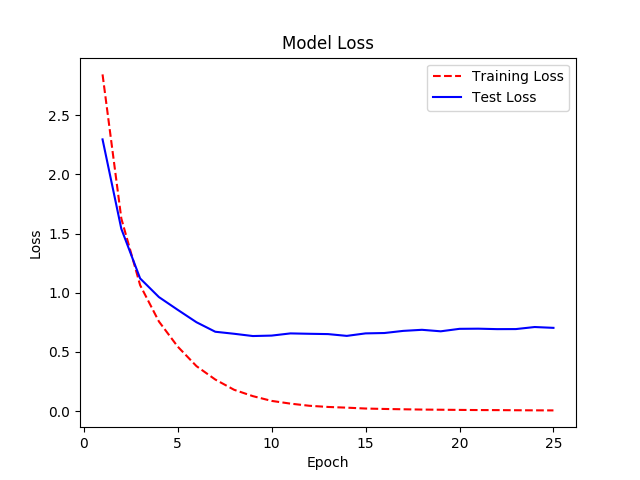
\includegraphics[scale=0.5]{images/OldModelLoss25Epochs.png}
    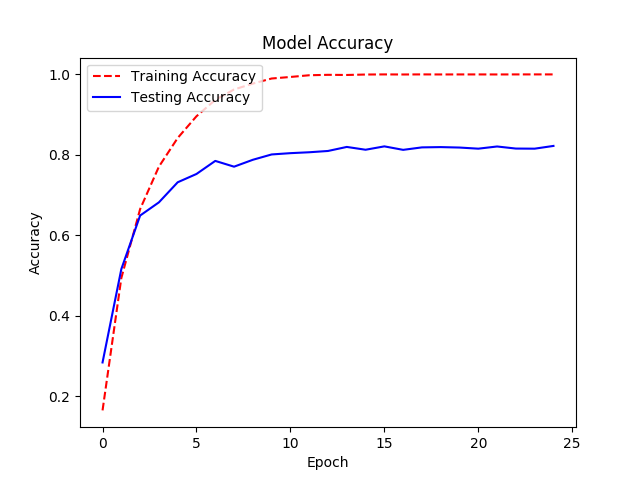
\includegraphics[scale = 0.5]{images/OldModelAccuracy25Epochs.png}
    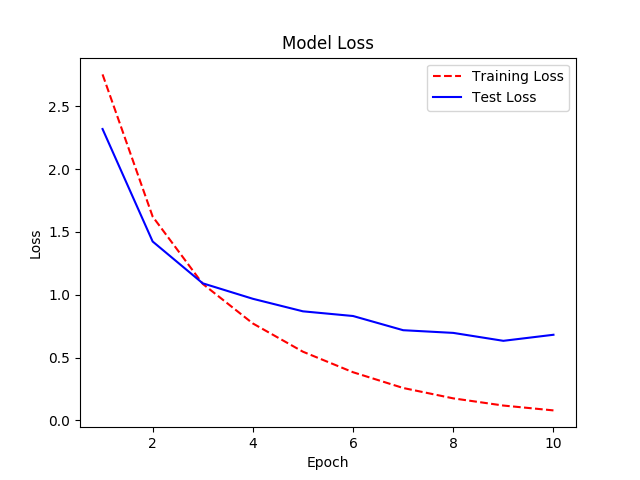
\includegraphics[scale=0.5]{images/OldModelLoss10Epochs.png}
    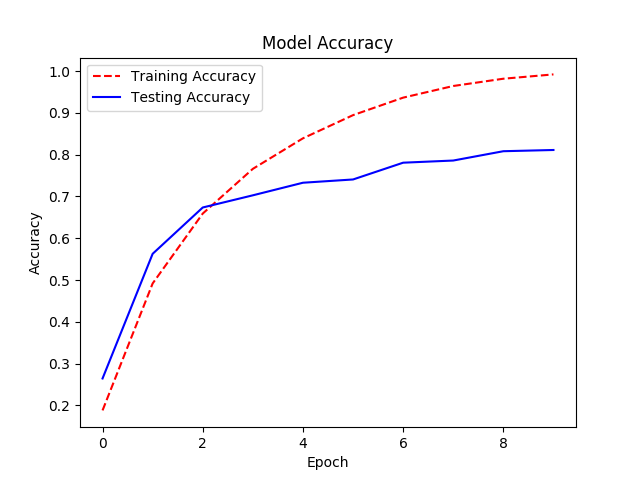
\includegraphics[scale = 0.5]{images/OldModelAccuracy10Epochs.png}
    \caption{Model Loss and Model Accuracy Charts for Old CNN for 100, 25, and 10 Epochs}
\end{center}
\end{figure}

For our "new" CNN, we used the same \textit{Model Loss} and \textit{Model Accuracy} charts to determine the optimal epoch count to train the network for, again aiming to avoid over-fitting the network to the training set. We again sought to find the epoch count at which accuracy reached a local maximum in the \textit{Model Accuracy} graph and at which value loss reached a local minimum. For the new CNN, we determined that this epoch count was at 7 epochs, as seen in the pairs of \textit{Model Loss} and \textit{Model Accuracy} charts for 100, 25, and 7 epochs below:

\begin{figure}[H]
\begin{center}
    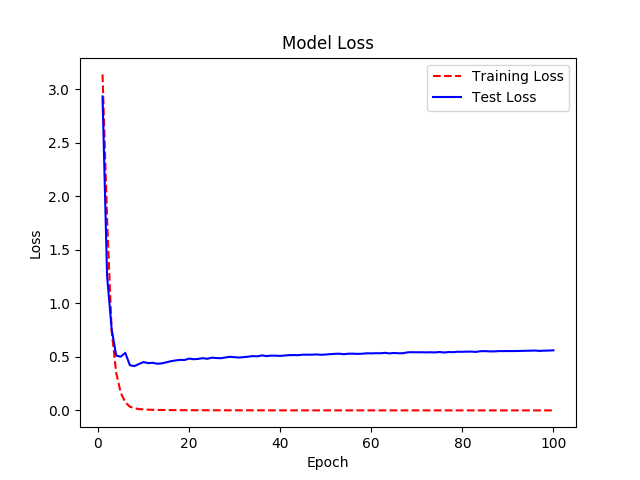
\includegraphics[scale=0.5]{images/NewModelLoss100Epochs.png}
    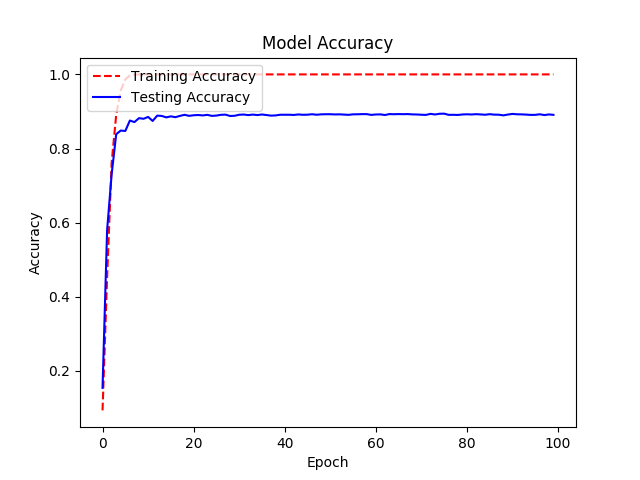
\includegraphics[scale = 0.5]{images/NewModelAccuracy100Epochs.png}
    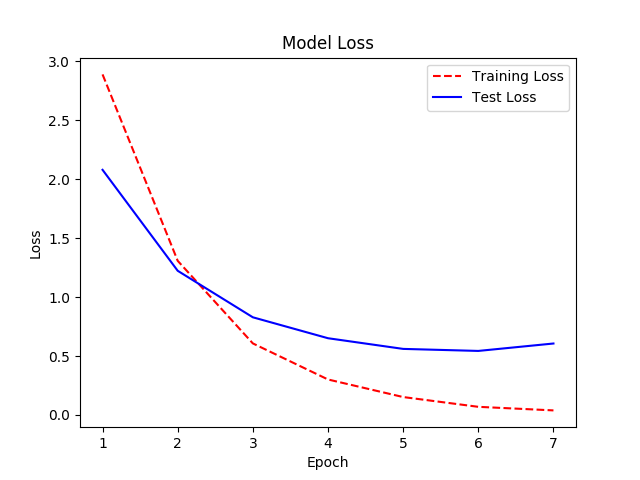
\includegraphics[scale=0.5]{images/NewModelLoss7Epochs.png}
    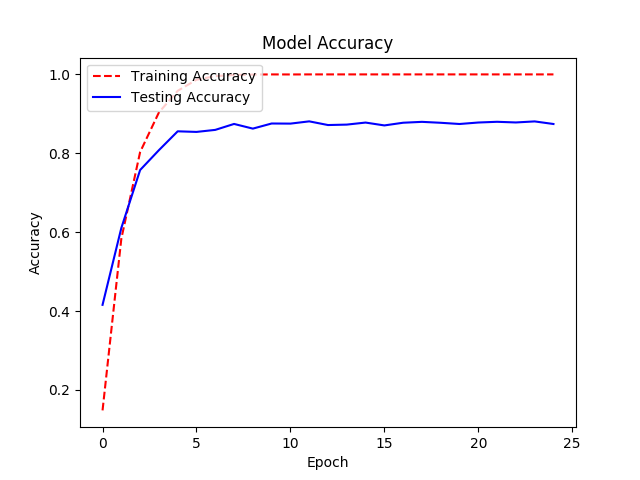
\includegraphics[scale = 0.5]{images/NewModelAccuracy25Epochs.png}
    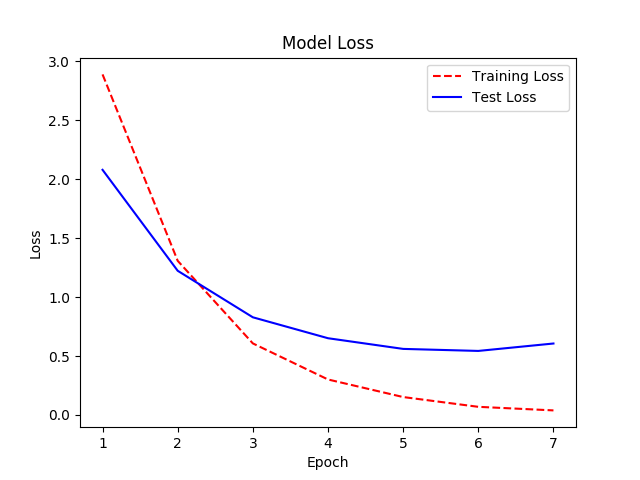
\includegraphics[scale=0.5]{images/NewModelLoss7Epochs.png}
    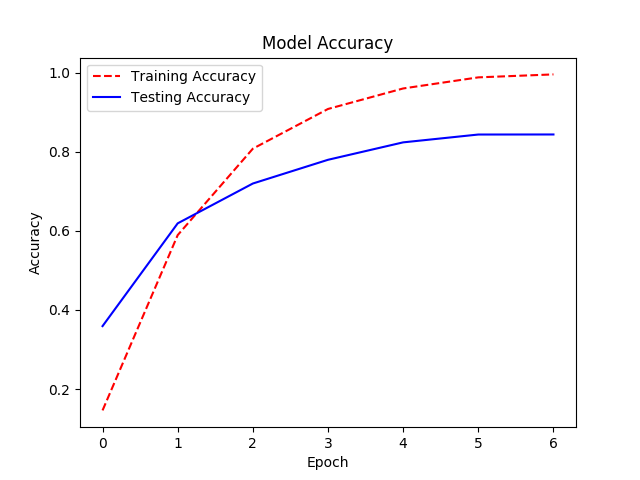
\includegraphics[scale = 0.5]{images/NewModelAccuracy7Epochs.png}
    \caption{Model Loss and Model Accuracy Charts for New CNN for 100, 25, and 7 Epochs}
\end{center}
\end{figure}

\section{Results}

We ran both of our convolution neural networks, the "old" one based off of the MNIST example from Lab 8 and the "new" one based off of the CNN shown in lecture for the MNIST example, five times each with the outlined parameters. The maximum accuracy rates across five runs for our old and new CNNs were 81.81\% and 89.14\%, respectively. The accuracy rates for each of the five runs, for both networks, and their averages are below:

\begin{figure}[H]
\begin{center}
\begin{tabular}{ |p{1.4cm}||p{1.8cm}|p{1.8cm}| }
 \hline
 \multicolumn{3}{|c|}{Accuracy Results} \\
 \hline
 \ Run \# & Old CNN Accuracy & New CNN Accuracy\\
 \hline
 \ \ \ \ 1 & \ \ 81.81\%    & \ \ 86.94\%\\
 \ \ \ \ 2 &  \ \ 79.45\% & \ \ 86.36\%  \\
 \ \ \ \ 3 & \ \ 79.63\% & \ \ 84.88\%\\
 \ \ \ \ 4 & \ \ 80.24\% & \ \ 87.46\%\\
 \ \ \ \ 5 & \ \ 80.07\% & \ \ 89.14\%\\
 \hline
 Average& \ \ 80.24\% & \ \ 86.95\%\\
 \hline
\end{tabular}
\caption{Accuracy Rates for Five Runs and Average Accuracy Rate for Old and New CNNs}
\end{center}
\end{figure}

We point out that the "new" CNN outperformed the "old" CNN in terms of average accuracy rate across five runs. In addition to seeing which CNN did better in terms of accuracy, we wanted to analyze which letters each network tended to mis-categorize or mis-predict. We did this via confusion matrices, at the suggestion of Professor Lisa Meeden. These matrices are 24x24, with integers representing the indices of each of the alphabet's letters (excluding 'j' and 'z' indexes of 9 and 25, respectively) populating the first row, and each of those integers populating the first column: these integers range from 0 to 24, excluding 9 as it is the index of 'j' in the alphabet. Each row element represents the actual letter the network attempted to predict, and each column element represents the letter predicted by the network. The intersection of the two contains the number of times the network mis-predicted the row element letter with the column element letter. In other words, by looking at the $i^{th}$ row and $j^{th}$ column, we see how many times during testing that the network incorrectly predicted the $j^{th}$ letter when the target letter was the $i^{th}$ letter. Below, we include the image of the ASL alphabet, included in the introduction, with labels of indexes; the numbers next to each sign in the image below match with the labels of the training and testing data. We also include the five-most frequent errors across one run of each CNN.

\begin{figure}[H]
\begin{center}
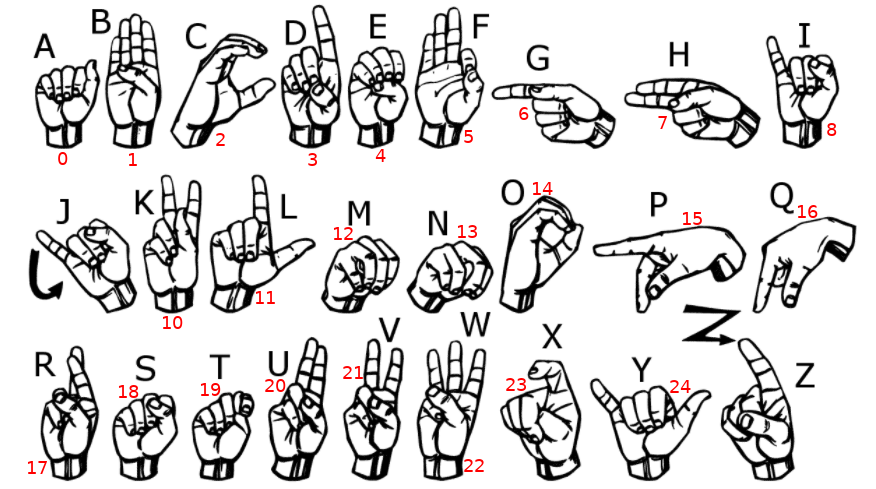
\includegraphics[scale=0.6]{images/Labeled_ASL_Alphabet.png}
\caption{ASL Alphabet, Labeled by Letter and Index Used by Data Set}
\end{center}
\end{figure}


\begin{figure}[H]
\begin{center}
\begin{tabular}{ |p{2.2cm}||p{1.8cm}|p{1.8cm}| }
 \hline
 \multicolumn{3}{|c|}{Old CNN's 5 Most-Frequent Errors} \\
 \hline
 \ Predicted \# & Actual \# & Frequency\\
 \hline
 \ \ \ \ 17 & \ \ 10 & \ \ 62\\
 \ \ \ \ 10 &  \ \ 20 & \ \ 56\\
  \ \ \ \ 23 & \ \ 19 & \ \ 55\\
 \ \ \ \ 4 & \ \ 18 & \ \ 41\\
 \ \ \ \ 16 & \ \ 6 & \ \ 41\\

 \hline
\end{tabular}
\caption{Old CNN's Five Most-Frequent Errors by Sign's Index in the ASL Alphabet}
\end{center}
\end{figure}


\begin{figure}[h]
\centering
\fbox{
\includegraphics{images/17-R.png}
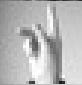
\includegraphics{images/10-K.png}}
\hspace{3mm}
\fbox{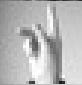
\includegraphics{images/10-K.png}

\includegraphics{images/20-U.png}}\\
\vspace{3mm}
\fbox{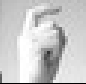
\includegraphics{images/23-X.png}

\includegraphics{images/19-T.png}}
\hspace{3mm}
\fbox{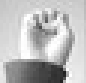
\includegraphics{images/4-E.png}

\includegraphics{images/18-S.png}}\\
\vspace{3mm}
\fbox{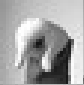
\includegraphics{images/16-Q.png}
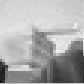
\includegraphics{images/6-G.png}}

\caption{Old CNN's Five Most Frequent Errors as Letter Pairs: (R(17), K(10)), (K(10), U(20)) (X(23), T(19)), (E(4), S(18)), (Q(16), G(6)), from Left-to-Right, Row-by-Row}
\end{figure}



\begin{figure}[H]
\begin{center}
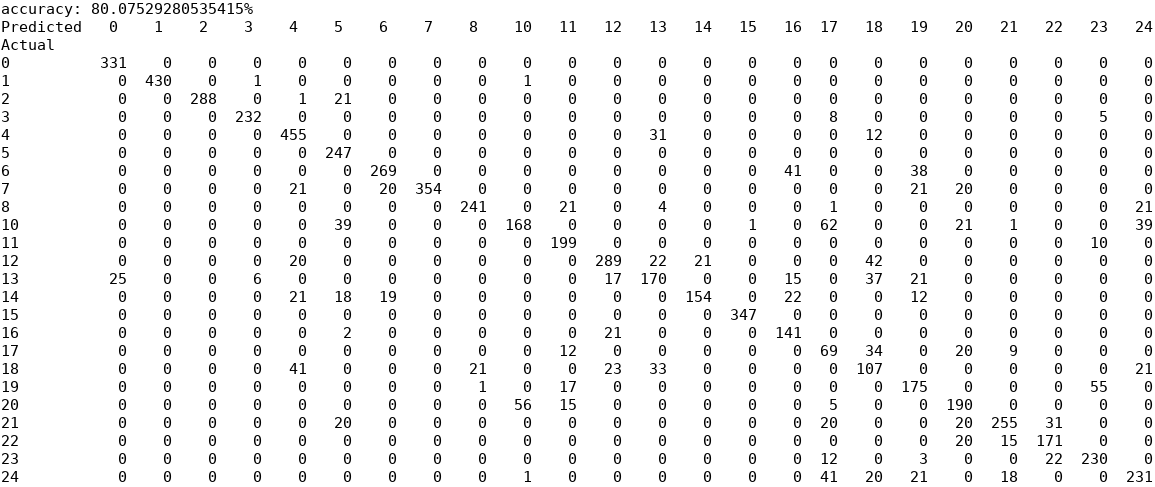
\includegraphics[scale=0.44]{images/Old_Confusion_Matrix_10Epochs.png}
\caption{Old CNN Confusion Matrix, Ten Epochs}
\end{center}
\end{figure}
% \vspace{10mm}

\begin{figure}[H]
\begin{center}
\begin{tabular}{ |p{2.2cm}||p{1.8cm}|p{1.8cm}| }
 \hline
 \multicolumn{3}{|c|}{New CNN's 5-Most Frequent Errors} \\
 \hline
 \ Predicted \# & Actual \# & Frequency\\
 \hline
 \ \ \ \ 23 & \ \ 19 & \ \ 62\\
  \ \ \ \ 16 & \ \ 13 & \ \ 42\\
   \ \ \ \ 20 &  \ \ 10 & \ \ 42\\
 \ \ \ \ 10 & \ \ 20 & \ \ 41\\
 \ \ \ \ 10 & \ \ 24 & \ \ 39\\
 \hline
\end{tabular}
\caption{New CNN's Five Most-Frequent Errors by Sign's Index in the ASL Alphabet}
\end{center}
\end{figure}

\begin{figure}[H]
\centering
\fbox{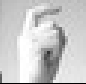
\includegraphics{images/23-X.png}

\includegraphics{images/19-T.png}}
\hspace{3mm}
\fbox{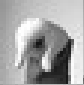
\includegraphics{images/16-Q.png}
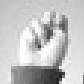
\includegraphics{images/13-N.png}}\\
\vspace{3mm}
\fbox{
\includegraphics{images/20-U.png}
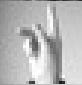
\includegraphics{images/10-K.png}}
\hspace{3mm}
\fbox{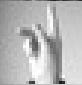
\includegraphics{images/10-K.png}

\includegraphics{images/20-U.png}}\\
\vspace{3mm}
\fbox{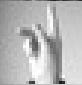
\includegraphics{images/10-K.png}

\includegraphics{images/24-Y.png}}

\caption{New CNN's Five Most-Frequent Errors as Letter Pairs: (R(17), K(10)), (K(10), U(20)) (X(23), T(19)), (E(4), S(18)), (Q(16), G(6)), from Left-to-Right, Row-by-Row}
\end{figure}

\begin{figure}[H]
\begin{center}
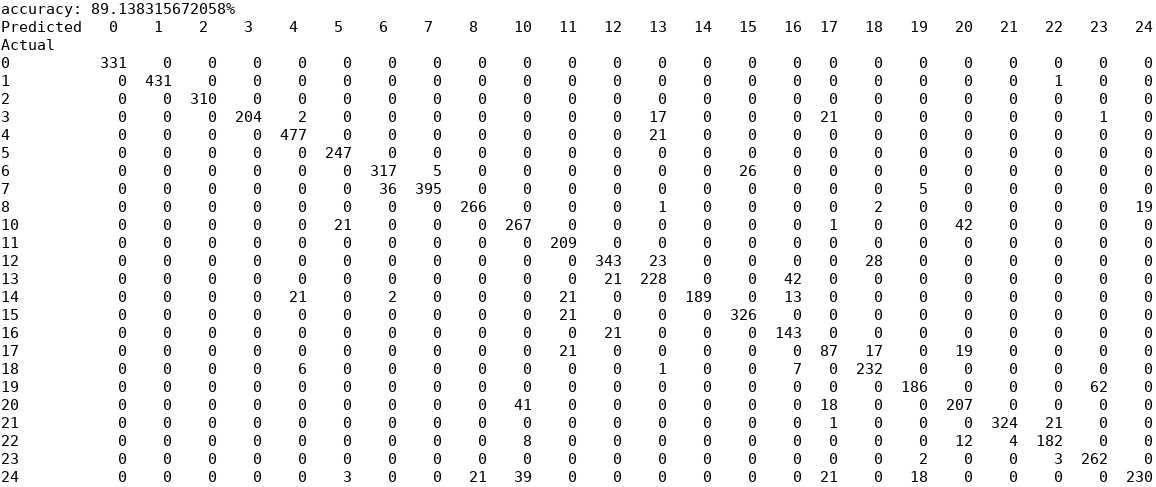
\includegraphics[scale=0.44]{images/Extra_Confusion_Matrix_7Epochs.png}
\caption{New CNN Confusion Matrix, Seven Epochs}
\end{center}
\end{figure}

Across both of our convolutional neural networks, the three most common incorrect predictions were between letters R(17) and K(10), X(23) and T(19), and K(10) and U(20)
As show by the pictures above, most errors occurred as a result of the target sign's image being nearly identical to what the CNN predicted: R(17) looks very
similar to K(10), for example, as do the other pairs of signs/letters shown in Figures 7 and 10. We assume that the features detected in such images corresponded well enough to the actual image that the CNN would predict incorrectly. Interestingly though, the "old" CNN confused the letter Q for the letter G a substantial
amount. This is despite the fact that the images shown vary greatly enough that features detected in the image would have little to no correlation. We
assumed that this was an edge case from one test run, but on multiple runs of our code, our CNN predicted Q for the letter G exactly 41 times on each run. On
the "new" CNN, this particular error no longer occurred, but a new curious error of Q being the predicted letter when the actual letter was N emerge. It also
predicted Q for N incorrectly 41 times on average.


\section{Conclusions}

The intent of this paper was to analyze how well CNNs can categorize images of signs from the ASL alphabet. Through our testing, we were able to see that even the most basic CNN yielded an average accuracy rate, across five runs, of 80.24\%. The inclusion of just one additional convolutional layer and one additional pooling layer, in the new CNN, improved the network's average accuracy rate to 86.95\%, an increase of approximately 6\%. This is due to the latter CNNs higher depth: it was able to detect more features than the old CNN and thus have a higher accuracy rate. We believe that a CNN can be a useful tool in categorizing ASL sign images based on these accuracy rates of greater than 80\%, but we still have some reservations. Our old CNN
had a unique error case in which the letter Q was consistently misinterpreted as the letter G (41 instances in one run). This translated over to our new CNN, where it consistently misinterpreted the letter Q as the letter N (42 instances in one run). This confusion between Q and G and between Q and N, in our old and new CNNs, respectively, was confusing as the corresponding images in the data set didn't seem to share many features; they weren't logical or easy-to-understand confusions based on the visual similarities between the signs for Q and those incorrect predictions. We saw that from our testing set, however, Q was one of the least occurring letters. We believed this played a part in this seemingly random error. Q, however, was one of the most occurring letters in the training set leaving us perplexed about what the CNN's were interpreting (Figure 12). Another potential cause of these errors involving the letter Q is the relatively strange orientation of Q's image that causes a larger shadow than other letters' images in the training and testing data. This error and our confusion surrounding it, however, evidences a primary weakness of CNNs. While the CNNs can accurately predict sign letters, we can't understand how or why the network made such predictions, which is especially pertinent in cases where the error isn't as trivial for humans to rationalize.



\begin{figure}[H]
\begin{center}
\begin{tabular}{ |p{2.7cm}||p{1.8cm}|}
 \hline
 \multicolumn{2}{|c|}{Training Letter Frequency} \\
 \hline
 \ Letter Index \# & Frequency \\
 \hline
 \ \ \ \ \ \ \ \ \ 0 & \ \ \ \ 1126 \\
 \ \ \ \ \ \ \ \ \ 1 & \ \ \ \ 1010 \\
 \ \ \ \ \ \ \ \ \ 2 &  \ \ \ \ 1144 \\
 \ \ \ \ \ \ \ \ \ 3 & \ \ \ \ 1196 \\
 \ \ \ \ \ \ \ \ \ 4 & \ \ \ \ \ 957 \\
 \ \ \ \ \ \ \ \ \ 5 & \ \ \ \ 1204 \\
 \ \ \ \ \ \ \ \ \ 6 & \ \ \ \ 1090 \\
 \ \ \ \ \ \ \ \ \ 7 & \ \ \ \ 1013 \\
 \ \ \ \ \ \ \ \ \ 8 & \ \ \ \ 1162 \\
 \ \ \ \ \ \ \ \ \ 10 & \ \ \ \ 1114 \\
 \ \ \ \ \ \ \ \ \ 11 & \ \ \ \ 1241 \\
 \ \ \ \ \ \ \ \ \ 12 & \ \ \ \ 1055 \\
 \ \ \ \ \ \ \ \ \ 13 & \ \ \ \ 1151 \\
 \ \ \ \ \ \ \ \ \ 14 & \ \ \ \ 1196 \\
 \ \ \ \ \ \ \ \ \ 15 & \ \ \ \ 1088 \\
 \ \ \ \ \ \ \ \ \boxed{16} & \ \ \ \boxed{1279} \\
 \ \ \ \ \ \ \ \ \ 17 & \ \ \ \ 1294 \\
 \ \ \ \ \ \ \ \ \ 18 & \ \ \ \ 1199 \\
 \ \ \ \ \ \ \ \ \ 19 & \ \ \ \ 1186 \\
 \ \ \ \ \ \ \ \ \ 20 & \ \ \ \ 1161 \\
 \ \ \ \ \ \ \ \ \ 21 & \ \ \ \ 1082 \\
 \ \ \ \ \ \ \ \ \ 22 & \ \ \ \ 1225 \\
 \ \ \ \ \ \ \ \ \ 23 & \ \ \ \ 1164 \\
 \ \ \ \ \ \ \ \ \ 24 & \ \ \ \ 1118 \\
 \hline
\end{tabular}\hspace{4mm}
\begin{tabular}{ |p{2.7cm}||p{1.8cm}|}
 \hline
 \multicolumn{2}{|c|}{Testing Letter Frequency} \\
 \hline
 \ Letter Index \# & Frequency \\
 \hline
 \ \ \ \ \ \ \ \ \ 0 & \ \ \ \ 331 \\
 \ \ \ \ \ \ \ \ \ 1 & \ \ \ \ 432 \\
 \ \ \ \ \ \ \ \ \ 2 &  \ \ \ \ 310 \\
 \ \ \ \ \ \ \ \ \ 3 & \ \ \ \ 245 \\
 \ \ \ \ \ \ \ \ \ 4 & \ \ \ \ 498 \\
 \ \ \ \ \ \ \ \ \ 5 & \ \ \ \ 247 \\
 \ \ \ \ \ \ \ \ \ 6 & \ \ \ \ 348 \\
 \ \ \ \ \ \ \ \ \ 7 & \ \ \ \ 436 \\
 \ \ \ \ \ \ \ \ \ 8 & \ \ \ \ 288 \\
 \ \ \ \ \ \ \ \ \ 10 & \ \ \ \ 331 \\
 \ \ \ \ \ \ \ \ \ 11 & \ \ \ \ 209 \\
 \ \ \ \ \ \ \ \ \ 12 & \ \ \ \ 394 \\
 \ \ \ \ \ \ \ \ \ 13 & \ \ \ \ 291 \\
 \ \ \ \ \ \ \ \ \ 14 & \ \ \ \ 246 \\
 \ \ \ \ \ \ \ \ \ 15 & \ \ \ \ 347 \\
 \ \ \ \ \ \ \ \ \boxed{16} & \ \ \ \boxed{164} \\
 \ \ \ \ \ \ \ \ \ 17 & \ \ \ \ 144 \\
 \ \ \ \ \ \ \ \ \ 18 & \ \ \ \ 246 \\
 \ \ \ \ \ \ \ \ \ 19 & \ \ \ \ 248 \\
 \ \ \ \ \ \ \ \ \ 20 & \ \ \ \ 266 \\
 \ \ \ \ \ \ \ \ \ 21 & \ \ \ \ 346 \\
 \ \ \ \ \ \ \ \ \ 22 & \ \ \ \ 206 \\
 \ \ \ \ \ \ \ \ \ 23 & \ \ \ \ 267 \\
 \ \ \ \ \ \ \ \ \ 24 & \ \ \ \ 332 \\
 \hline
\end{tabular}
\caption{Letter Frequency in Training and Testing Data, Each Index Refers to Sign Letter's Index in ASL Alphabet (Q Index and Frequencies are Boxed)}
\end{center}
\end{figure}

\end{document}
